\documentclass[twocolumn,11pt]{article}
\usepackage{authblk}
\usepackage{graphicx}
\usepackage{hyperref}
\usepackage{amsmath}
\usepackage{lipsum,adjustbox}
\usepackage{tikz}
\usetikzlibrary{calc, positioning}


\title{Tor Inter-Relay Latency}
\author[1]{Frank Cangialosi}
\author[1]{Scott DellaTorre}
\author[1]{Emily Kowalczyk}
\author[1]{Brent Schlotfeldt}
\author[1]{Dave Levin\thanks{Faculty Advisor}}
\affil[1]{University of Maryland}
\date{}
\raggedbottom

\renewcommand{\thefootnote}{\fnsymbol{footnote}}

\begin{document}
\maketitle

\section {Introduction}

The Internet, once a small network of hosts operated primarily by large academic and governmental institutions, has grown dramatically in the decades since its conception. The result, an exceedingly complex network comprised of billions of intercommunicating hosts, is much more difficult to analyze than the system from which it evolved. At the same time, the importance of such analysis is perhaps greater now than it ever was. Millions of people have become daily users of the Internet, relying on the network to quickly access information and communicate with their peers. Less frequent users number in the billions, and thousands more gain Internet access every day. As network designers, engineers, and researchers strive to accommodate the ever-increasing demands of these and future users, their success will depend in part on their ability to determine the current state of the network. Indeed, the designers of the future Internet will need to recognize and address problems that the network currently faces, and be able to adapt their solutions in response to changing network conditions. In pursuit of these goals, their access to comprehensive and up-to-date network statistics will be essential.

Unfortunately, gathering this information on a large scale is difficult. Although there exist many tools to measure network statistics, they require direct access to a source host. For example, \texttt{ping} and \texttt{traceroute}--networking utilities which provide useful information such as network latency, packet loss, and the route taken by packets--do so by sending small data packets from an originating host to a destination host. Thus, tools such as these can only generate measurements that originate from a controlled source. This requirement hinders the ability of  researchers to compute comprehensive network statistics. Indeed, a researcher is limited both by the number of host machines to which he or she has access and the locations of these hosts. Using existing tools, a researcher cannot choose two arbitrary hosts, or even two arbitrary locations, and determine the network conditions between them. If we could provide researchers this ability, it would greatly expand their access to global network conditions, allowing them to produce much more comprehensive analyses of the global Internet than are currently possible.

Of course, access to arbitrary hosts on the Internet is not a feasible goal. This would require every user to volunteer a portion of their network bandwidth to research, a contribution only a small fraction of users would likely be willing to make. Nevertheless, by tapping into this collection of volunteered hosts, we can achieve a much more refined picture of the global Internet. Researchers have used this strategy in past studies, taking network measurements using hosts volunteered to PlanetLab, a group of computers available as a test bed for computer networking and distributed systems research, as well as other public clusters \cite{PlanetLab}. However, the vast majority of hosts in such clusters are administered by large corporations and academic institutions. These organizations connect to the Internet in very different ways than an average home user does. For one, they typically have much faster networks, many more users sharing the network connection at once, and much more complicated network configurations than home users do, all of which can greatly influence network measurements. These organizations also usually have different providers and links to the Internet than home users do. For example, many academic institutions have access to high-speed academic networks such as Internet2 in the U.S. and G\'EANT in Europe \cite{Geant}. Additionally, corporations sometimes peer with one another, agreeing to route each other’s traffic for free. Evidently, there are many differences between home networks and the networks of corporations and universities. Thus, measurements from hosts in clusters like PlanetLab do not accurately portray the network conditions observed by millions of home users.

To fill in this gap, we propose taking network measurements between computers volunteered by home users. Fortunately, such a network, Tor, already exists. Tor is an anonymity network comprised of over four thousand routers, known as Tor relays \cite{Tor}. The routers are run by volunteers from around the world, many of whom are simply running the Tor relay software on their home computers. If we could take network measurements using these relays, we could produce useful statistics for average home network connections, something which we could not do using PlanetLab or similar clusters. However, Tor was not designed for the purpose of network measurement, so using the network in this regard is not entirely straightforward.

Nevertheless, we devise a method which uses the Tor network to measure network conditions among its relays. We apply this method to measure a specific network statistic, round-trip time (RTT), between two arbitrarily-chosen Tor relays. Our insight is that the full RTT measurement between a source and destination host represents the sum of the latencies between each host in the path, plus forwarding delays for each Tor relay. As we discuss in more detail in a later section, we can achieve our desired result with knowledge only of the full RTT for and a few related RTTs. Making use of this observation, we develop a tool that computes network latency between Tor relays, and use this tool to measure the RTT between two arbitrarily selected relays. In doing so, we demonstrate the feasibility of capturing network conditions for the average home user.

The remainder of our paper progresses as follows. In section 2, we provide a brief overview of the Tor network, which we used to carry out our experiments. In section 3, we discuss related works which pursue network measurement between arbitrary hosts, as well as works which aim to measure network statistics specifically on Tor. We give a more detailed description of our algorithm in section 4, and describe the methods we used to collect our measurements. In section 5, we present and analyze the results generated by our tool for a particular pair of Tor relays. Finally, in section 6, we conclude and discuss future work.

\section{Tor Network}

In this section, we provide a brief overview of how the Tor network operates in order, introduce terminology needed for later sections of the paper, and  the properties of Tor which allow for isolation of the RTT between two hosts. 

The Tor client anonymizes a host's traffic by securely rerouting its Internet transactions. Rather than connecting directly to a website, for example, a host sends its request through a series of Tor ``relays,'' which are simply other hosts whose owners have chosen to volunteer bandwidth to the Tor network. According to the Tor Metric Portals, the network currently contains over 4,700 such relays \cite{Tor_Metrics_Portal}.

A series of connected relays is known as a ``circuit.'' When initialized, the Tor client uses a path selection algorithm to construct circuits, each containing at least three relays. In order to create these circuits, the client extends its path, one relay at a time, exchanging a unique set of encryption keys with each new relay. The circuit design ensures that each individual relay can determine only the immediate source and destination of a packet. The Tor client uses a minimum of three relays in each circuit, ensuring no intermediary router can discover both the original source and final destination of a packet sent through the Tor network. \footnote[1]{Assuming the relays in the circuit are administered independently, and the relay administrators do not collude to break this anonymity.} Although any relay may be used within a circuit, the final relay must be an ``exit relay,'' as designated by its operator. Only exit relays can deliver traffic to and from the final destination host \cite{tor_about}.

To boost anonymity further, the Tor client uses each circuit for a maximum of ten minutes before switching to an entirely new one. This measure limits the amount of data an eavesdropping relay operator can collect about a Tor user. Additionally, the Tor software allows any application to utilize its anonymous connection by providing a SOCKS interface. Users commonly employ Tor to anonymize their network traffic for activities such as IRC chat messaging, web browsing, and DNS lookups \cite{tor_about}.


\section{Related Work}

Several existing studies have explored the problem we presented--namely, the measurement of network conditions between arbitrarily selected hosts. Just as we did, Gummadi et al. undertook the measurement of network latencies between arbitrarily selected hosts, though through entirely different means \cite{Gummadi}. They present a tool, King, which estimates the network latency between two given hosts by determining the latency between two DNS name servers, one nearby each host. King determines the latency between the DNS servers using a novel insight: by simply sending a recursive request to one DNS server for a name over which the other DNS server has authority, they can force the first server to send and receive data from the second server, allowing them to compute the RTT between the servers. An evaluation of King demonstrates that its latency estimates are very accurate in the majority of cases. However, as the researchers acknowledge, the measurements King provides are indeed only estimates, their accuracy largely dependent upon the proximity of each host to a cooperating DNS server. In cases where a host is not very close to a DNS server or the DNS server closest to it does not resolve recursive requests, King fails to produce an accurate estimate. Nonetheless, King compensates for its weaknesses by alerting its user when it fails, or has likely failed, to produce an accurate estimate.

Wang et al. expand upon the work done by Gummadi et al. to create a tool that estimates packet loss between arbitrary hosts--another goal aligned with our broad objective of determining network conditions among hosts we cannot directly control \cite{Wang}. Their tool, Queen, finds DNS servers close to the specified hosts and forces them to communicate, borrowing King's recursive query technique. They then estimate the packet loss between the two servers using another novel insight about DNS servers: the packet loss rate between two DNS servers can be inferred based on the latency measured between the two servers. The researchers determined each server's retransmission rate beforehand by forcing it to retransmit repeatedly until it reached its retry limit. With the knowledge of the retransmission rates, they were able to accurately estimate how many queries and DNS server responses were lost, based on the observed round-trip latencies of the queries and responses. Wang et al. used this data to estimate the packet loss rate between the original hosts, an approximation which they verified was quite accurate in most cases.

Eriksson et al. accurately estimate yet another network statistic between arbitrary host pairs: hop distance, or the number of routers on the path between the hosts \cite{Eriksson}. They do so by inserting a number of ``landmark nodes'' throughout the Internet. These nodes learn about the Internet topology in two ways: by actively probing one another, and by passively monitoring network packet traffic. By utilizing passive measurements, the researchers limit the number of active measurements they need, reducing the overhead introduced by the landmark nodes. Eriksson et al. demonstrate their ability to accurately estimate the number of hops between arbitrary nodes in the network, using the collected active and passive data in conjunction with a multidimensional scaling algorithm they devised. They further enhance this approximation by analyzing passively-collected BGP data.

Each aforementioned research group presents an innovative method, as well as an accompanying tool which implements it, to estimate a network statistic between arbitrary hosts connected to the Internet. Furthermore, each team verifies that their tool can produce reasonably accurate results for the majority of host pairs. However, the presented solutions differ from our own in that they do not involve sending data between the selected hosts. Conceivably, two hosts could experience dramatic packet loss or network latency when trying to communicate, while the network conditions appeared fine between the DNS servers or landmark nodes nearby. By resolving to compute network latency through direct measurements, we reduce the probability that we will overlook an important network anomaly. However, the requirement for direct measurements also limits the number of host pairs we can analyze. Undoubtedly, each method of measurement has its merits, and each has its downfalls. To achieve the most widespread understanding of global Internet conditions, we should develop tools of both varieties.

A few other network statistics tools, designed specifically for the Tor network, share many implementation details with our own tool. For example, Tor-RTT is a tool which measures round-trip times for Tor connections \cite{Tor_RTT}. However, Tor-RTT is limited to measuring the RTT for the entire circuit, not the inter-relay RTTs we seek to measure. Nevertheless, we build upon the techniques used by Tor-RTT in our own implementation; we discuss the distinction in more detail in section 4. Another related work, Tor Metrics Portal, is a public database which stores useful statistics regarding the composition and performance of the Tor network \cite{Tor_Metrics_Portal}. The portal measures several statistics for Tor relays over time, such as read-to-write ratio, download performance, and bandwidth utilization; it also stores information about the clients who use these relays. However, the portal does not, to our knowledge, store any data regarding inter-relay latencies. Hence, we present a novel technique to compute this measure.

\section{Procedure}

As previously mentioned, our procedure is founded upon our observation that the total RTT for data sent between two hosts in the Tor network is simply the sum of a number of measurable components. Specifically, it comprises the individual RTTs between each pair of consecutive nodes in the connection (the source, the destination, and the relays which connect them), as well as the forwarding delays ($F_x$) for each Tor relay in the circuit. Knowing this, we can intelligently construct specific circuits, measure the total RTT for each of them, and then perform some simple algebraic operations to isolate a single inter-relay RTT, as desired.


\definecolor {processblue}{cmyk}{1,1,1,1}

\definecolor{green}{HTML}{218559}
\definecolor{blue}{HTML}{336699}
\definecolor{orange}{HTML}{B06A3B}
\definecolor{red}{HTML}{DD1E2F}
\begin{figure*}
\centering
\begin{adjustbox}{width=\textwidth}
\begin {tikzpicture}[-latex ,auto ,node distance =2.5cm and 2.5cm ,on grid ,
semithick ,
state/.style ={ circle ,top color =white , bottom color = gray!20 ,
draw,processblue , text=black , minimum width =1 cm}]
\node[state] (S)
{$S$};
\node[state] (W) [above right =of S] {$W$};
\node[state] (X) [right =of W] {$X$};
\node[state] (Y) [right =of X] {$Y$};
\node[state] (Z) [right =of Y] {$Z$} ; 
\node[state] (D) [below right =of Z] {$D$};
\path ([xshift=-1.5ex,yshift=3ex]S.east) edge node[above left = .2 cm] {$R_{sw}$} ([xshift=.25ex,yshift=-1.25ex]W.west);
\path ([xshift=.25ex,yshift=-1.25ex]W.west) edge  ([xshift=-1.5ex,yshift=3ex]S.east);
\path[color=orange] ([xshift=-.5ex,yshift=1.5ex]S.east) edge ([xshift=1.25ex,yshift=-2.75ex]W.west);
\path[color=orange] ([xshift=1.25ex,yshift=-2.75ex]W.west) edge node[below right = 0.25cm]{$R_{sw}$} ([xshift=-.5ex,yshift=1.5ex]S.east);

\path[color=blue] (S) edge[bend right = 20] node[below right = 0.3cm]{$R_{sy}$} (Y);
\path[color=orange] (X) edge[bend right = 20] (D);
\path[color=blue] (Y) edge[bend right = -20] (S);
\path[color=orange] (D) edge[bend right = -20] node[below left = 0.3cm]{$R_{xd}$} (X);
\path[color=blue] ([yshift=-1ex]Y.east) edge ([yshift=-1ex]Z.west); 
\path[color=blue] ([yshift=-1ex]Z.west) edge node[below = 0.3cm]{$R_{yz}$} ([yshift=-1ex]Y.east); 
\path[color=blue] ([xshift=0ex,yshift=1ex]D.west) edge ([xshift=-1ex,yshift=-2ex]Z.east);
\path(S)[color=red] edge [bend left = 100] node[above left = .3cm]{$R_{sy}$} (Y);
\path[color=orange] ([yshift=-1ex]W.east) edge node[below  = 0.3cm]{$R_{wx}$} ([yshift=-1ex]X.west);
\path[color=orange] ([yshift=-1ex]X.west) edge ([yshift=-1ex]W.east);
\path ([yshift=.5ex]X.west) edge node[above = .3 cm] {$R_{wx}$}([yshift=.5ex]W.east);
\path ([yshift=.5ex]W.east) edge ([yshift=.5ex]X.west);
\path (X) edge [bend left =0] node[above = .3 cm] {$R_{xy}$}(Y);
\path (Y) edge [bend right =0](X);
\path ([yshift=.5ex]Y.east) edge [bend left =0] node[above = .3 cm] {$R_{yz}$}([yshift=.5ex]Z.west);
\path ([yshift=.5ex]Z.west) edge ([yshift=.5ex]Y.east);
\path (Z.east) edge [bend left =0] node[above right = .3 cm] {$R_{zd}$}([xshift=1.5ex,yshift=2.5ex]D.west);
\path ([xshift=1.5ex,yshift=2.5ex]D.west) edge [bend right =0](Z.east);
\path[color=green] (D) edge [bend right=100]  node[above right = .3cm]{$R_{wx}$} (X);
\path[color=blue] ([xshift=-1ex,yshift=-2ex]Z.east) edge node[below left = 0.3cm]{$R_{zd}$} ([xshift=0ex,yshift=1ex]D.west);
\path[color=blue] ([xshift=0ex,yshift=1ex]D.west) edge ([xshift=-1ex,yshift=-2ex]Z.east);
{\tiny }\end{tikzpicture}
\end{adjustbox}
\caption{S and D represent the source host (our local computer) and the destination host (bluepill.cs.umd.edu), respectively, while W, X, Y, and Z represent four arbitrary Tor relays. Each distinctly colored path represents a different circuit whose RTT is measured.}
\end{figure*}

Although we intend to calculate the RTT between two arbitrary hosts which we do not administer, we still need control over two other hosts in order to send data through the targeted relay pair. For this experiment, we use a local machine connected to the Tor network as a source host (S) for communications, and a University of Maryland server, bluepill.cs.umd.edu, as a destination host (D) for receiving these connections. On our destination server, we deploy a simple program written in Python. This program listens for incoming TCP connections on a particular port and responds to two types of queries received from the source host. For ``echo'' queries, the server responds by simply repeating the received message back to the source. For ``ping'' queries, the server responds with the resulting latencies measuring by a series of pings to a specified host.
	
On our source host, we run another program, also written in Python, which employs the Stem library in order to construct and monitor specific Tor circuits. Additionally, we make use of the SocksiPy library to easily create sockets which use Tor as a proxy server. Although the Stem library provides functionality for custom circuit creation, it still leaves path selection up to the Tor network, which uses its own algorithm to determine the best path from the list of generated circuits. In order to manually force Tor to use a specific circuit for data transmission, we emulate a technique used by the Tor-RTT tool \cite{Tor_RTT}; namely, we listen to our controller for stream events, attaching a stream to the current circuit whenever a new stream is created. Using this technique for circuit creation and selection, our client performs the following original procedure to determine the round-trip time between two hosts, X and Y:

\begin{enumerate}
\item Create a circuit of four randomly chosen Tor nodes, W, X, Y, and Z, from a list of operating exit relays (retrieved from \href{http://torstatus.blutmagie.de}{http://torstatus.blutmagie.de})
\item Send a 64-byte message from S to D, through the circuit W, X, Y, Z, (the black path in Figure 1), and measure the total RTT as $T_{wxyz}$, defined as:
\begin{align*}
T_{wxyz} &= R_{sw} + R_{wx} + R_{xy} + R_{yz} + R_{zd} \\
  &\quad + F_w + F_x + F_y + F_z
\end{align*}
\item Create a circuit containing only the first two nodes in the original four-node circuit, W and X
\item Send a 64-byte message from S to D, through the circuit W, X (the brown path in Figure 1), and measure the total RTT as $T_{wx}$, defined as:
\[\color{orange} 
T_{wx} = R_{sw} + R_{wx} + R_{xd} + F_w + F_x
\]
\vspace{-.7cm}
\item Create a circuit containing only the last two nodes in the original four-node circuit, Y and Z
\item Send a 64-byte message from S to D, through the circuit Y, Z (the blue path in Figure 1), and measure the total RTT as $T_{yz}$, defined as:
\[\color{blue}
T_{yz} = R_{sy} + R_{yz} + R_{zd} + F_y + F_z
\] 
\vspace{-.7cm}
\item Manually ping the IP address of relay X from Bluepill (D) to find $\color{green} R_{xd}$
\item Manually ping the IP address of relay Y from our source computer (S) to find $\color{red} R_{sy}$
\item Make the following final calculation:
\begin{align*}
& R_{wxyz} - \color{orange}R_{wx} \color{black}- \color{blue}R_{yz} \color{black}+ \color{red}R_{sy} \color{black}+ \color{green}R_{xd} \\
&\quad = (\color{black} R_{sw} + R_{wx} + R_{xy} + R_{yz} + R_{zd} \\&\quad + F_w + F_x + F_y + F_z) \\
&\quad - (\color{orange} R_{sw} + R_{wx} + R_{xd} + F_w + F_x\color{black}) \\
&\quad - (\color{blue} R_{sy} + R_{yz} + R_{zd} + F_y + F_z\color{black})\\
&\quad + (\color{green} R_{xd}\color{black}) + (\color{red} R_{sy}\color{black}) \\
& = R_{xy}
\end{align*}
\end{enumerate}

\newpage

\begin{figure*}[t!]
\centering
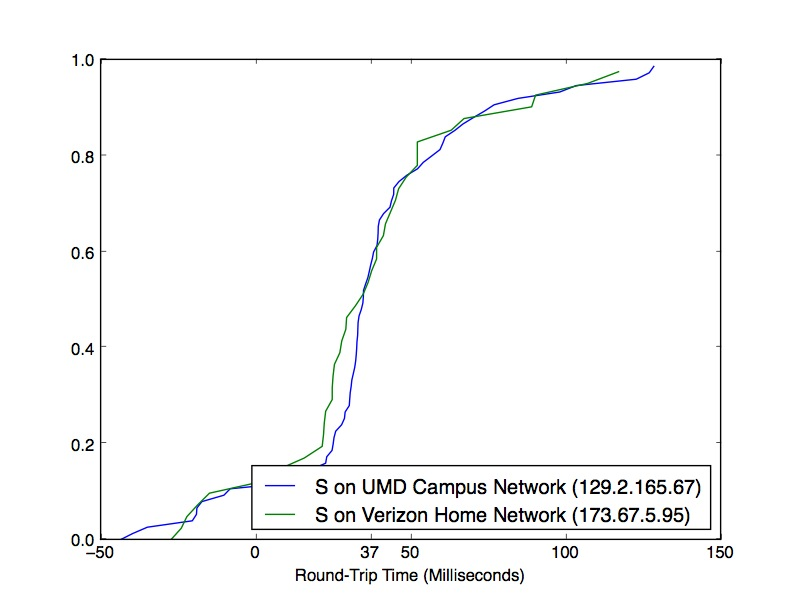
\includegraphics[width=4in]{cdf}
\caption{\label{fig:myfigure} CDF of arbitrarily changing W and Z, while leaving X and Y constant measured by host S on two different different networks.}
\end{figure*}

\section{Evaluation}

Although we eventually intend to use our tool to collect large datasets of the latencies between all relays on the Tor network, and potentially to track this information continually over time, our current study focuses on analyzing the accuracy of the data our tool collects, to first ensure that it will be reliable enough for these purposes.

We test the accuracy of our tool by constructing circuits on S in which we keep the X and Y relays constant and randomly choose different pairs of W and Z relays. We conjecture that the calculated value of $R_{xy}$ will be similar for each circuit, and thus, independent of any changes made to S, W, Z, or D, since all of the round-trip and forwarding delay components involving these hosts are eliminated by the final calculation. Further, we expect $R_{xy}$ to be independent of the network to which S is connected.

In order to test our hypotheses, we first arbitrarily select X and Y from a list of valid exit nodes to be 213.239.214.175, located in Nuremberg, Germany, and 62.149.13.57, located in Kiev, Ukraine. Additionally, we connect S to the University of Maryland wireless network. We then create 50 circuits on S, selecting two other relays at random to represent W and Z. For each of these 50 circuits, we take 10 measurements at each step of the procedure; in the last step, we use these results to compute 10 possibilities for the value of $R_{xy}$. Of these 10 values, we choose the median--the statistic which appears to provide the most consistent estimate of the actual RTT. Figure 2 displays a cumulative distribution function of the fifty resulting medians. Finally, we repeat the above trials, this time with S connected to a Verizon home network in Ellicott City, MD; we plot the CDF of these results in Figure 2 as well.

In both cases, we find that a majority of the trials produced results near 37 milliseconds. Although we cannot directly confirm this value without controlling X and Y, the geographic distance between X and Y, roughly 944 miles, suggests that a 37-millisecond RTT is plausible. However, we also acknowledge that there are a number of outliers in our data. Considering a study conducted by Chen and Pasquale \cite{improving_path}, which found that latencies in the Tor network were highly variable, it seems likely that the variation in our calculations stems from inconsistencies in the network rather than bugs in our tool. Although a single run of our tool may not produce an accurate value for the RTT between X and Y--in fact, the final estimate for $R_{xy}$ is occasionally negative--a series of runs over time produce a clear trend centered around a specific, and reasonable, value. Factors such as the fluctuating demands of Tor users on the network's relays could potentially explain the high degree of variability in our results.

\section{Conclusion}

In this paper, we present a novel approach to collecting latency measurements between two hosts we do not control. Additionally, we present a tool which employs our approach to measure latencies between relays in the Tor network. Although our tool requires these hosts to be exit relays in the Tor network, this still provides more than one thousand widely spread nodes to choose from. Furthermore, many of these relays belong to basic home networks; these provide insight into the conditions of home network connections, links which tend to be less accessible for analysis. Compared to other tools involving network measurement between arbitrary hosts, our tool differs in that it measures along the actual path between hosts, rather than an approximate path; in doing so, it captures network conditions that these related tools might miss. While network statistics tools and databases exist for Tor, none that we know of allows the measurement of inter-relay latencies, or any inter-relay statistic. While our results demonstrate that single runs of our tool do not always provide accurate measurements--potentially due to high variability within the Tor network--we found that the distribution of many individual results centered around a reasonable value.

Due to the novelty of our method, there are a great number of possible directions for future work. One potential advancement could be the collection of RTTs for all pairs of exit nodes in the Tor network. Given the number of exit nodes currently in operation, this would require calculations for about 500,000 different pairs--a fairly large undertaking, but one which could feasibly be completed in a reasonable time frame. If our method could be modified to calculate RTTs between \textit{any} two relays in the Tor network, this would enable measurements between more than 12 million pairs of relays, significantly increasing the amount of accessible network data. Applying our technique to measure other network statistics, such as packet loss, could provide important new data as well. Ultimately, much work remains to be done in the field of network analysis, as we strive to improve our understanding of the ever-changing Internet.
 
\bibliography{biblio}
\bibliographystyle{abbrv}

\end{document}
